% ########################################################################################################################################
%
% This is the main latex file. Here we call for inputs from other files. We also define some of the main characteristics of the document.
%
% ########################################################################################################################################
%
% You likely only need to modify the "Main_Content__Write_your_essay_here.tex" file.
%
% ########################################################################################################################################

\documentclass[12pt,a4paper,oneside]{paper}
%TC:ignore
% ################################################################################
% 
%       INSTRUCTIONS, PLEASE READ BEFORE IF YOU INTEND TO MODIFY THIS FILE
% 
% ################################################################################
% For the most part, you should not change this file. In particular, the format 
% should not be changed. However, depending on what you want you might need to
% use additional packages (and possibly remove old ones that may be incompatible.
% Do that at your own discretion.
% ################################################################################

% Encoding and Language
\usepackage[utf8x]{inputenc}
\usepackage{csquotes}
\usepackage[main=portuguese]{babel}
\usepackage{iflang}

% Font Configurations
\renewcommand{\rmdefault}{phv}
\renewcommand{\sfdefault}{phv}
\def\FontLn{% 16 pt normal
  \usefont{T1}{phv}{m}{n}\fontsize{14pt}{14pt}\selectfont}
\def\FontLb{% 16 pt bold
  \usefont{T1}{phv}{b}{n}\fontsize{14pt}{14pt}\selectfont}
\def\FontMn{% 14 pt normal
  \usefont{T1}{phv}{m}{n}\fontsize{12pt}{12pt}\selectfont}
\def\FontMb{% 14 pt bold
  \usefont{T1}{phv}{b}{n}\fontsize{12pt}{12pt}\selectfont}
\def\FontSn{% 12 pt normal
  \usefont{T1}{phv}{m}{n}\fontsize{10pt}{10pt}\selectfont}

% Font Encoding
\usepackage[T1]{fontenc}

% Page Geometry
\usepackage{geometry}	
\geometry{verbose,tmargin=2cm,bmargin=1.7cm,lmargin=2cm,rmargin=2cm}
\usepackage{multirow}
\usepackage{multicol}

% Line Spacing
\usepackage{setspace}
\renewcommand{\baselinestretch}{1.2}

% Graphics and Figures
\usepackage{graphicx}
\usepackage{subfigure}
\usepackage{subfigmat}
\usepackage{float}

%Colors
\usepackage{xcolor}

% Mathematics and Theorems
\usepackage{amsmath}
\usepackage{amsthm}
\usepackage{amsfonts}
\usepackage{dcolumn}
\usepackage{indentfirst}

% Comments and Verbatim
\usepackage{verbatim}

% Hyperlinks
\usepackage[pdftex]{hyperref}
\hypersetup{
    colorlinks,
    linkcolor=blue,
    anchorcolor=black,
    citecolor=cyan,
    filecolor=black,
    menucolor=black,
    urlcolor=teal,
    bookmarksopen=true,
    bookmarksnumbered=true
}

% Captions and References
\usepackage[figure,table]{hypcap}
\usepackage[format=plain]{caption}
\DeclareCaptionFont{georgia}{\small\fontseries{n}\fontfamily{georgia}\selectfont}
\captionsetup{labelfont=georgia,font=georgia}

% Bibliography
\usepackage[backend=biber,style=apa]{biblatex}

% Index
\usepackage{makeidx}
\makeindex

% Acronyms
\usepackage[printonlyused]{acronym}

% Lipsum (for placeholder text)
\usepackage{lipsum}

% Cleveref (for clever references)
\usepackage[\IfLanguageName{english}{english}{portuguese}]{cleveref}

% Colors
\usepackage{xcolor}
\usepackage{color}

% Custom Commands
\newcommand{\gray}[1]{\textcolor{gray}{#1}}

% Equation Numbering
\renewcommand{\theequation}{{\fontseries{n}\fontfamily{georgia}\selectfont\arabic{equation}}}

% Section and Subsection Fonts
\sectionfont{\Large\bfseries\fontfamily{lmss}\selectfont}
\subsectionfont{\large\bfseries\fontfamily{lmss}\selectfont}
%TC:endignore


\addbibresource{bibliography.bib}
\begin{document}
\pagestyle{fancy}
\fancyhf{} % Clear previous settings
\rhead{LIFE}
\lhead{Espetroscopia e Efeito Fotoelétrico}

%TC:ignore
% #############################################################################
%
%                           ENTER YOUR NAME, ISTid, AND TITLE
% 
% #############################################################################



\def\title {}


% #############################################################################
%
%               DO NOT MODIFY THE LINES FROM HERE TO THE MAIN DOCUMENT BODY
% 
% #############################################################################

\thispagestyle {empty}
\begin{center}
\begin{minipage}[c][5cm][t]{\textwidth}
\begin{center}

\includegraphics[width=5cm]{../IST_A_RGB_POS.png}
\end{center}

\end{minipage}
\begin{minipage}[t][10cm][c]{\textwidth}
\centering
{\FontMb Instituto Superior Técnico} \\
\paragraph{}
\centering
{\FontLb\Huge \title{}}
\paragraph{}
\centering
{\FontMb Laboratório de Introdução à Física Experimental} \\
\paragraph{}
{\FontMb 2023/2024}
\end{minipage}

\begin{minipage}[c][2cm][c]{\textwidth}
\centering
{\FontLn }
\end{minipage}
\begin{minipage}[c][2cm][c]{\textwidth}
\centering
\end{minipage}
\begin{minipage}[c][1cm][c]{\textwidth}
\centering
\fbox{{\FontMb Report}}
\end{minipage}
\begin{minipage}[c][3cm][c]{\textwidth}
\centering
{\FontMb
102716 Pedro Curvo}
\end{minipage}
\begin{minipage}[c][2cm][c]{\textwidth}
\centering

\end{minipage}

\end{center} 
\normalsize
\cleardoublepage
\setcounter{page}{1}
\fontfamily{cmr}\selectfont
%TC:endignore
% #############################################################################
%
%                           BEGIN MAIN DOCUMENT BODY
%
% #############################################################################

\printindex


%%%%%%%%%%%%%%%%%%%%%%%%%%%%%%%%%%%%%%%%
\section{\sf Conceitos fundamentais}
\subsection{\sf Desvio da luz por um prisma}
Em óptica designa-se por \emph{prisma} um sólido transparente em forma de prisma triangular, homogéneo e isotrópico,
caracterizado pelo ângulo do vértice $\alpha$ e pelo índice de refração $n$. Quando colocado no percurso de um feixe luminoso
incidente, o prisma produz um desvio angular no feixe emergente que depende do ângulo de incidência e do comprimento de onda
$\lambda$ (Fig. \ref{fig:prisma1}). Na região da luz visível, verifica-se que os comprimentos de onda mais curtos são mais
desviados, ou seja, a luz violeta é mais desviada que a luz vermelha.

\begin{figure}[htb]  \centering 
	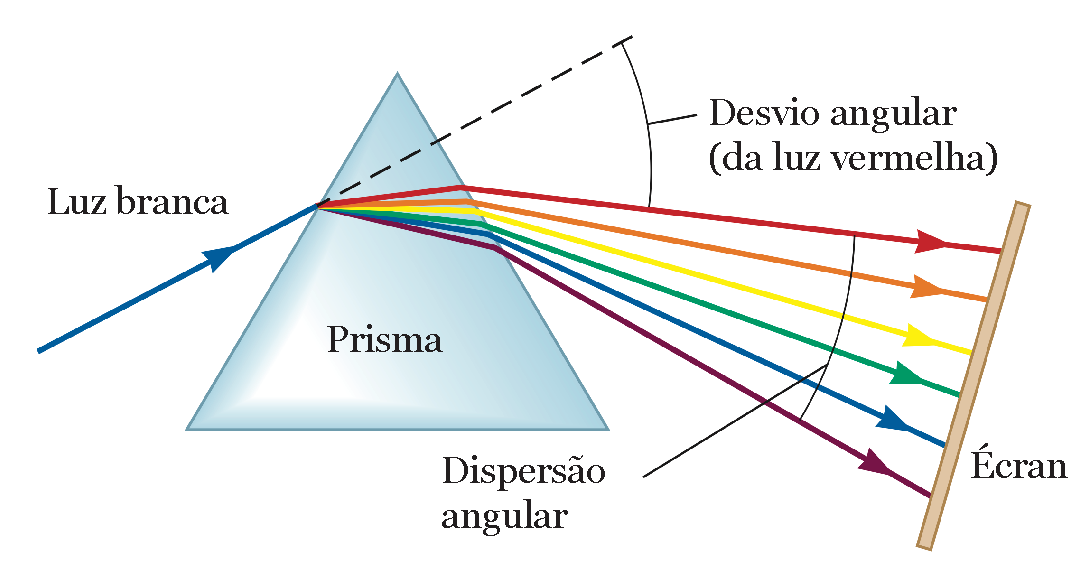
\includegraphics[width=0.5\textwidth]{./planck_images/prisma1.pdf}
	\caption{Desvio da luz por um prisma: um feixe de luz branca é desviado da sua direcção original de um ângulo que
	depende do ângulo de incidência e do comprimento de onda. \label{fig:prisma1}} 
\end{figure}

A Fig. \ref{fig:prisma2} mostra este processo em maior detalhe. Um raio luminoso (traço vermelho contínuo) incide na face
esquerda do prisma segundo um ângulo $i_1$ (em relação à normal à superfície) e é refractado internamente segundo um ângulo $t_1$. Após se propagar dentro do prisma, o raio incide na face direita segundo um ângulo $i_2$ e é refractado para o exterior segundo um ângulo $t_2$. À diferença entre a direcção original e a desviada chamamos \emph{desvio angular} $\delta(\lambda)$. Pode provar-se que a função $\delta(\lambda)$ apresenta um ponto estacionário (i.e., derivada nula) que é um mínimo se $n > 1$. Mostra-se também que, nessa situação, as direções dos dois feixes são igualmente inclinadas em relação às faces do prisma, i.e.  o ângulo de incidência $i_1$ é igual ao ângulo de transmissão emergente $t_2$. Nesse caso, o índice de refração, $n$, pode ser calculado simplesmente através da expressão seguinte: 

\begin{equation}
	\label{eq:desviomim}
	n= \frac{\sin \left( \frac{\alpha+ \delta_{min}}{2} \right) } {\sin \left(  \frac{\alpha}{2} \right)}  
\end{equation}
em que $\alpha$ e  $\delta_{min}$ são o ângulo do vértice do prisma e o \emph{ângulo de desvio mínimo} referido,
respectivamente. Uma vez que o índice de refracção depende $\lambda$, podemos concluir que também o valor de $\delta_{min}$
vai depender do comprimento de onda: diferentes cores vão apresentar diferentes desvios mínimos. Este princípio permite,
através da medição do desvio mínimo $\delta_{min}(\lambda)$ para vários comprimentos de onda, determinar por ajuste a variação
do índice de refracção do material do prisma.


\begin{figure}[htb]  \centering 
	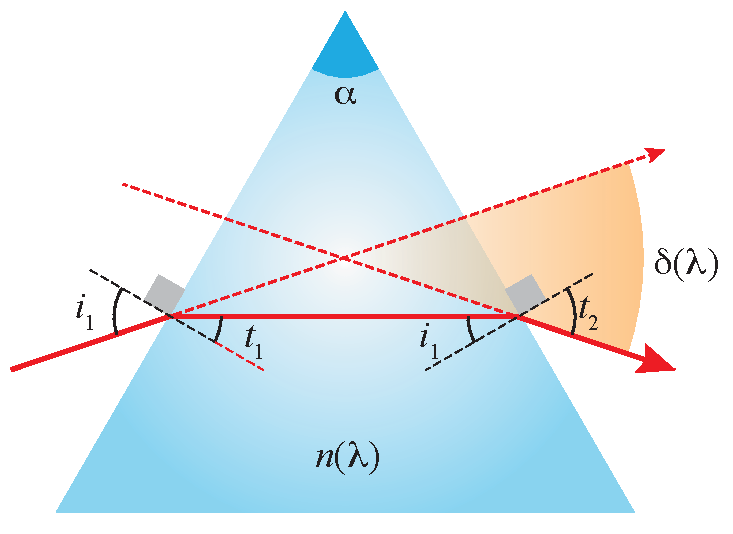
\includegraphics[width=0.5\textwidth]{./planck_images/prisma2.pdf}
	\caption{Definição de \emph{ângulo de desvio} $\delta(\lambda)$. A luz viaja da esquerda para a direita através de um
	prisma de índice de refracção $n(\lambda)$ e ângulo de vértice $\alpha$. \label{fig:prisma2}} 
\end{figure}

\subsection{\sf Rede de difracção}
Uma rede de difracção é um componente óptico com uma estrutura microscópica periódica – por exemplo, pode ser composto por
fendas paralelas (linhas) com espaçamentos da ordem do micrómetro. Caracteriza-se a rede pelo número $N$ de linhas por mm,
que é assim da ordem de várias centenas, ou mesmo superior. Tal como o prisma, a rede tem a propriedade de desviar a luz
incidente em função do ângulo de incidência e do comprimento de onda $\lambda$, só que duma forma muito mais apreciável.
Um raio de luz de c.d.o. $\lambda$ que incida com um ângulo $\theta_i$ (relativamente à normal) numa rede de difracção com
$N$ linhas/mm é difractado segundo um ângulo $\theta_d$, de acordo com
\begin{equation}
\sin \theta_i+\sin\theta_d=m \lambda N
\end{equation}
em que $m$ é a \emph{ordem de difracção}. A Fig. \ref{fig:rede1} ilustra a difracção para o caso em que o ângulo de incidência
é nulo, isto é, o feixe incide segundo a normal à superfície. O feixe central, não desviado, é considerado como $m=0$, enquanto
que à esquerda e direita surgem simetricamente as ordens $m=\pm 1, \pm 2$, etc., cada vez menos intensas.

\begin{figure}[!t]  
\centering 
	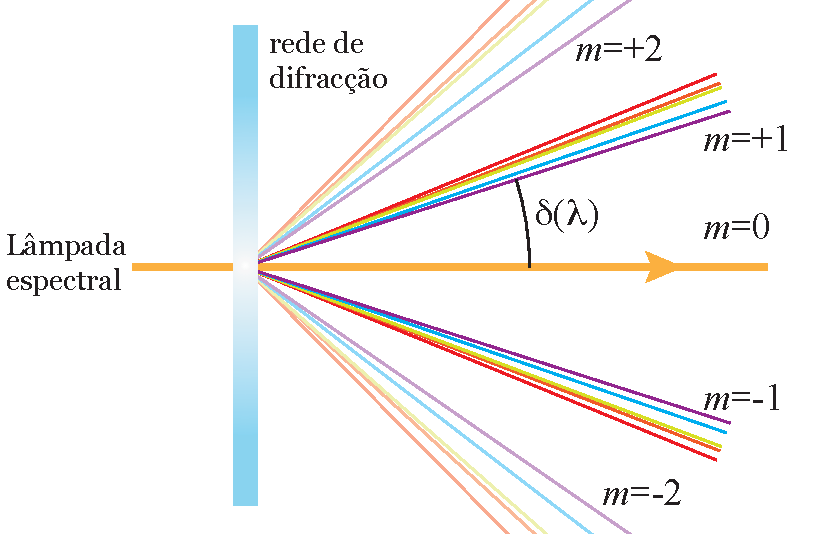
\includegraphics[width=0.5\textwidth]{./planck_images/rede1}
	\caption{Desvio da luz por uma rede de difracção, com o surgimento de ordens de difracção. \label{fig:rede1}} 
\end{figure}


\section{\sf Goniómetro de Babinet}
O goniómetro é um instrumento que permite medir ângulos com grande precisão, e muito utilizado em óptica. O goniómetro de
Babinet tem uma base central quase cilíndrica com uma plataforma que roda em torno do eixo vertical daquela, na qual é colocado
o elemento dispersor da luz (prisma ou a rede de difracção) (Figura \ref{fig:goniometer}). 

O goniómetro vem equipado com dois elementos ópticos: um \emph{colimador} e uma \emph{luneta}. Ambos estão montados radialmente,
o colimador fixo e a luneta podendo rodar em torno do eixo da base (Figura \ref{fig:babinet}). As posições angulares da plataforma
(e, portanto, do prisma ou da rede) e da luneta podem ser lidas num limbo graduado por intermédio de nónios solidários, respetivamente
com a plataforma e a luneta. Existem dois parafusos micrométricos, cada um associado a cada um dos nónios, que permitem com facilidade
regular e fazer leituras das posições angulares, com resolução de $30''$ (meio minuto de grau).

\begin{figure}  
\centering 
	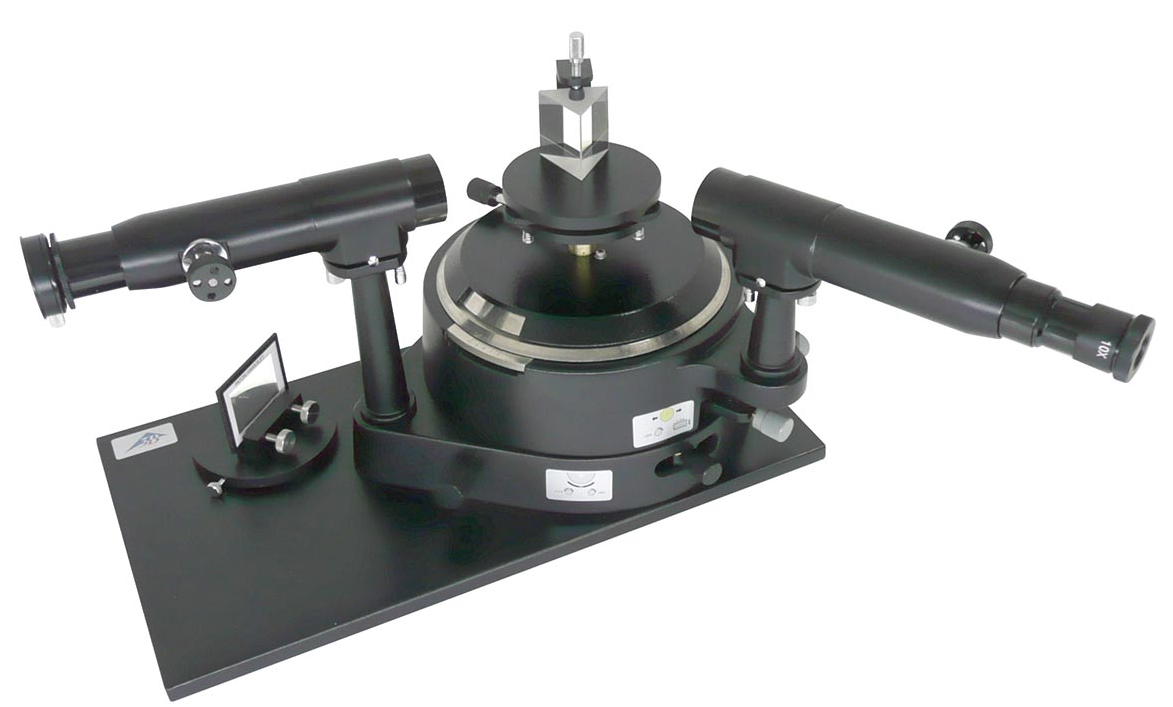
\includegraphics[width=0.75\textwidth]{./planck_images/goniometer}
	\caption{Goniómetro de Babinet . \label{fig:goniometer}} 
\end{figure}

O \emph{colimador} é constituído por dois tubos cilíndricos concêntricos que se podem deslocar axialmente. Um deles possui uma
fenda rectilínea, de largura variável por um parafuso, e que deve ser colocada na vertical (pode utilizar a mira da ocular depois
de regulada) e encostada à fonte luminosa. O outro tubo tem no extremo oposto (virado para a plataforma) uma lente convergente,
$L_C$. O objectivo deste conjunto é produzir um feixe de raios paralelos na região da plataforma onde se coloca o prisma, rede,
ou espelho. A fenda, se for relativamente estreita, vai funcionar como objecto linear e dar origem às riscas observadas.

\begin{figure}
	\centering 
	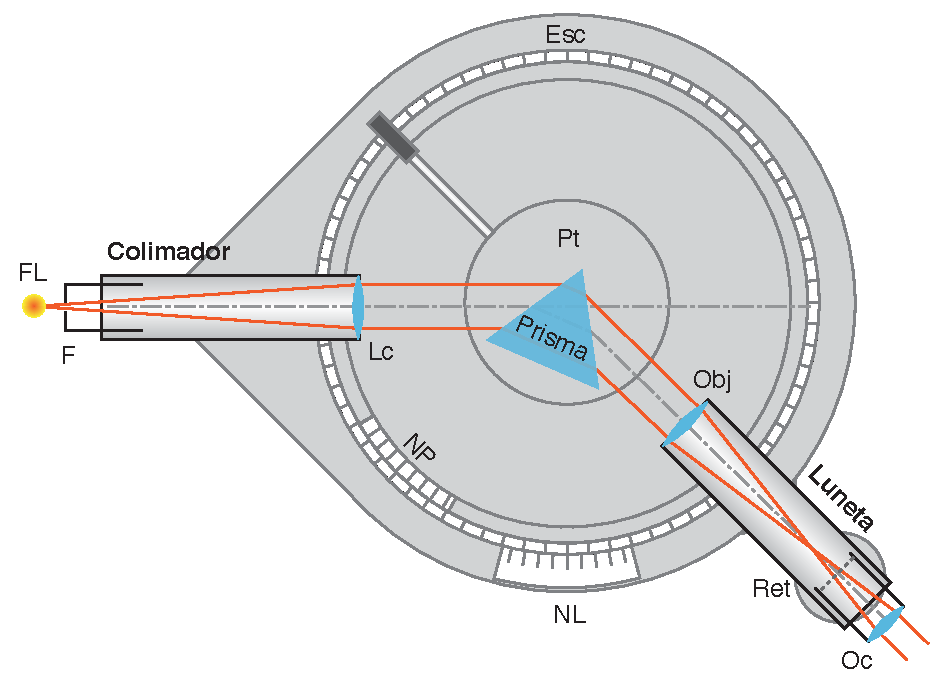
\includegraphics[width=0.65\textwidth]{./planck_images/Babinet}
	\caption{Esquema do goniómetro. FL -- fonte luminosa, F -- fenda, Lc -- lente convergente, Pt -- plataforma, Esc -- escala
	fixa na base, NL -- nónio acoplado ao suporte da luneta, NP -- nónio acoplado ao suporte do prisma, Obj -- objetiva, Oc -- ocular,
	Ret -- retículo.
	\label{fig:babinet}} 
\end{figure}

A \emph{luneta} é constituída por dois elementos ópticos, uma lente convergente e uma ocular munida de retículo
(dois fios cruzados perpendicularmente). A primeira lente produz no seu plano focal a imagem intermédia da fenda,
que é projectada no plano do retículo e ampliada pela ocular. A ocular é regulada pelo observador, de modo a ver uma
imagem focada da fenda.

\subsection{\sf Leitura de valores no goniómetro}
O goniómetro tem uma escala central, fixa e solidária com a base, com valores entre $0^\circ$ e $360^\circ$. Entre cada
grau há três divisões, ou seja, a escala está dividida em intervalos de 1/3 grau = 20 minutos de arco (20')
(Fig. \ref{fig:gonio-nonio1}). Existem duas escalas rotativas com um nónio: a de cima está unida à plataforma e permite
ler o ângulo de incidência, a de baixo está ligada à luneta e permite ler o ângulo de desvio. Estes ângulos são relativos,
por exemplo, à direcção do feixe de luz sem sofrer desvio. Ambas as escalas móveis estão equipadas com nónios de 40 divisões,
aumentando assim a precisão da leitura para 20'/40=0.5', ou seja, 30 segundos de arco. O uso desta precisão é facultativo nas
medições feitas com a rede (dada a amplitude dos ângulos de desvio) mas é obrigatório para medições com o prisma.

\begin{figure}
	\centering 
	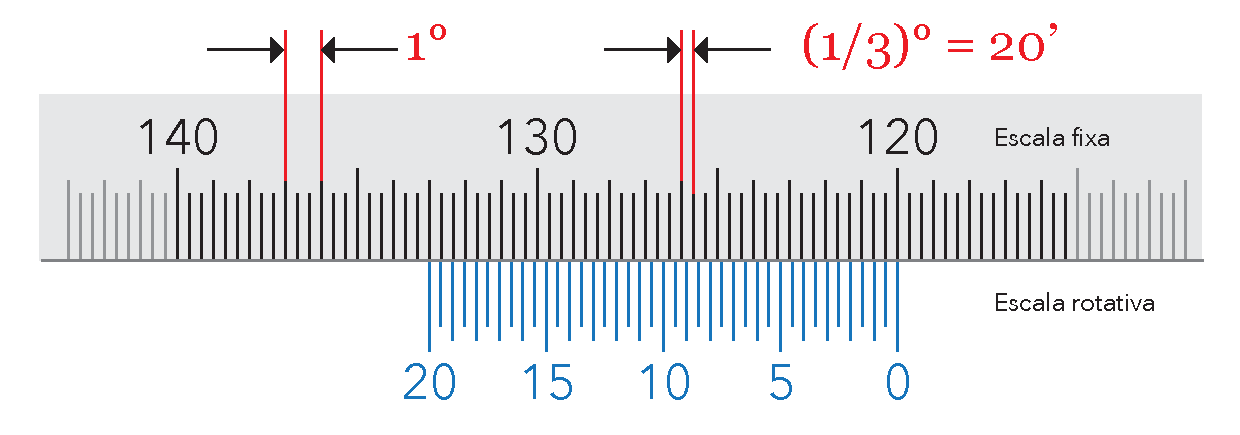
\includegraphics[width=0.5\textwidth]{./planck_images/gonio-nonio1}
	\caption{Escala fixa (menor divisão: 20') e escala rotativa, com nónio, do goniómetro.
	\label{fig:gonio-nonio1}} 
\end{figure}

O procedimento para ler um dado valor usando o(s) nónio(s) é semelhante ao usado na craveira (Fig. \ref{fig:gonio-nonio2}).
Começa-se por ler na escala fixa, com a maior precisão possível, o valor imediatamente à esquerda da linha do zero do nónio.
A esse valor acrescenta-se o valor indicado pela divisão cuja linha coincide em ambas as escalas. Dado o tamanho diminuto
destas divisões, é aconselhável fazer a leitura com o auxílio de uma lupa, ou registar a leitura através de fotografia digital
(Fig. \ref{fig:gonio-lente}).

\begin{figure}[h]
	\centering 
	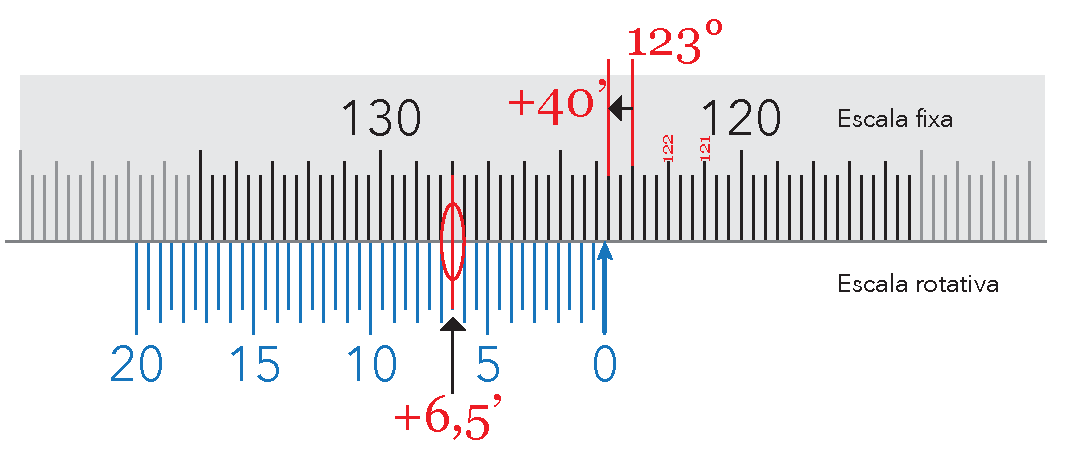
\includegraphics[width=0.5\textwidth]{./planck_images/gonio-nonio2}
	\caption{Exemplo de leitura no goniómetro. Escala fixa: $123^\circ+40'$; nónio: 6,5'. Valor da leitura: $123^\circ46,5'$
	\label{fig:gonio-nonio2}} 
\end{figure}

\begin{figure}[h]
	\centering 
	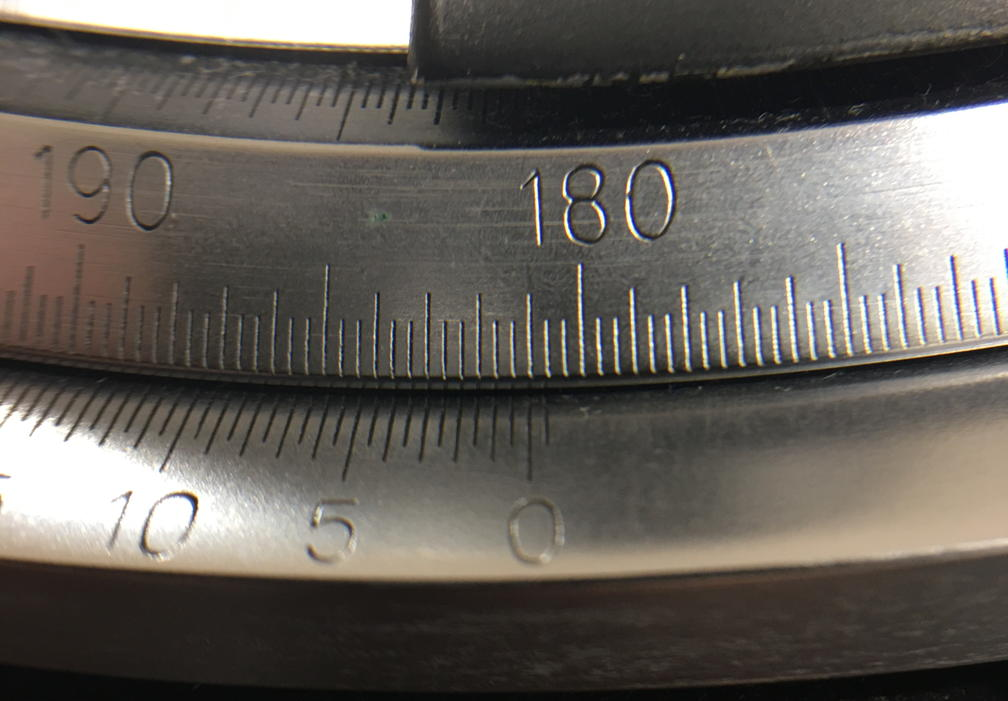
\includegraphics[width=0.4\textwidth]{./planck_images/gonio-lente}
	\caption{Registo em fotografia digital auxiliado por lente da leitura do goniómetro.
	\label{fig:gonio-lente}}
\end{figure}

Por outro lado, o valor que é lido nas duas escalas do goniómetro – escala da plataforma e escala da luneta – não coincide
necessariamente com o ângulo de incidência ou o ângulo de desvio, respectivamente, o que pode levar a confusão no registo dos
valores. A Fig. \ref{fig:babinet3} ilustra esta situação para o caso da refracção no prisma. Por uma questão de consistência,
iremos utilizar a seguinte convenção:

\begin{itemize}
\item Os ângulos de incidência e transmissão nos componentes ópticos, relativamente às suas superfícies, são designados $\theta_i$ e $\theta_t$ respectivamente
\item Os ângulos lidos na escala da plataforma e na escala da luneta são designados $\phi_i$ e $\phi_t$ respectivamente; 
\item O ângulo lido na escala da luneta na ausência de componente óptico é $\phi_{i0}$; nessa configuração a luneta encontra-se
perfeitamente alinhada com o colimador
\end{itemize}

De novo considerando a Fig. \ref{fig:babinet3}, para o caso do prisma pode deduzir-se a seguinte relação entre
$\phi_{i0}$, $\phi_t$ e o ângulo de desvio:
\begin{equation}
\delta=|\phi_{i0}-\phi_t |
\end{equation}

\begin{figure}[h]
	\centering 
	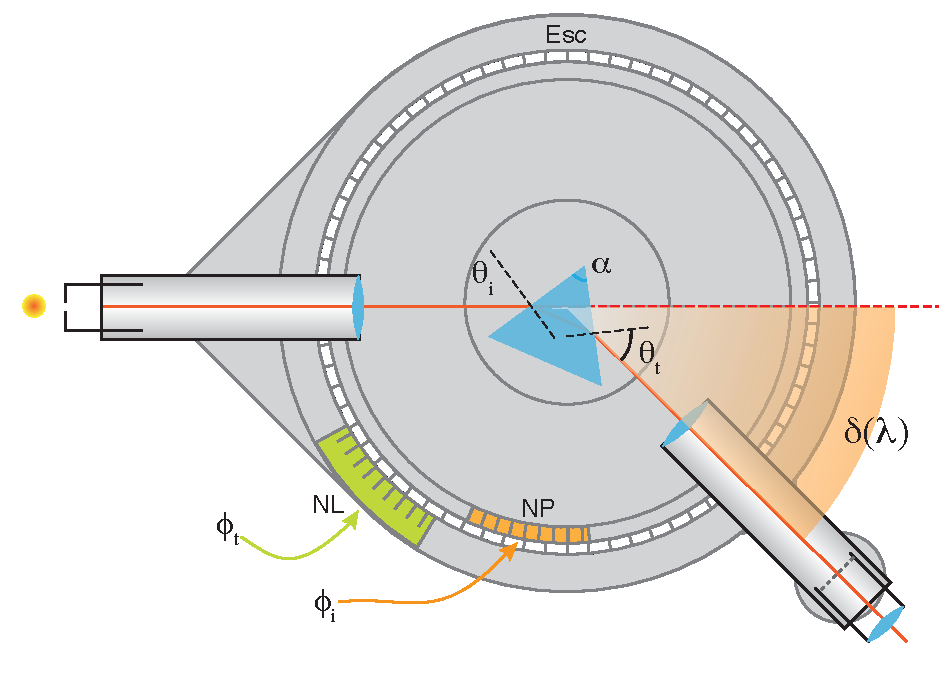
\includegraphics[width=0.6\textwidth]{./planck_images/Babinet3}
	\caption{Identificação dos diversos ângulos na refracção da luz por um prisma.
	\label{fig:babinet3}} 
\end{figure}




\newpage


\section{\sf Efeito fotoeléctrico}
O efeito fotoeléctrico era já conhecido no final do séc. XIX, com a emissão  de partículas carregadas da superfície de um
metal quando iluminadas por luz intensa. Verificou-se também que a energia destas partículas, que mais tarde foram identificadas
por electrões, não dependia da intensidade da luz incidente mas sim do  seu comprimento de onda, $\lambda$.  A explicação correcta
do efeito fotoeléctrico foi proposta em 1905 por Albert Einstein\footnote{Pela qual recebeu o prémio Nobel em 1921.} baseada na
teoria de Max Planck\footnote{Teoria Quântica da luz, pela qual recebeu o prémio Nobel em 1918.} da emissão-absorção da luz.
Para ambos, a luz seria formada pela emissão de  corpúsculos (\emph{quanta}), que se batizaram como \emph{fotões}, cada um
com energia $E$  dada por $E = h \nu$, em que $h$ é apropriadamente a \emph{constante de Planck} e $\nu$ a frequência da luz
($\nu=c/\lambda$).  De acordo com esta teoria corpuscular da luz, quando um fotão incide sobre a superfície de um metal é
absorvido por um átomo, e a sua energia é depositada num dos electrões de valência.
% A estes electrões tem de ser depositada uma energia para que se libertem da rede metálica. 
 Se o fotão incidente tiver mais energia que um dado limiar ($W_0$ - \emph{Work function}, característica de cada metal),
 o  electrão é libertado da rede metálica e emitido do sólido com uma energia cinética $K_e = h\nu - W_0$.
A intensidade da luz determina assim o \emph{número de fotolectrões} emitidos, mas não a sua energia!

A Fig. \ref{fig:pe-effect} representa esquematicamente o efeito. Os fotões incidentes, de energia $h\nu$, libertam electrões
próximos da superfície do sólido. Note-se que se a energia do fotão incidente não for suficiente (i.e. se $E_f < W_0$) não
há emissão de fotoelectrões.

\begin{figure}[htb] 
	\centering 
	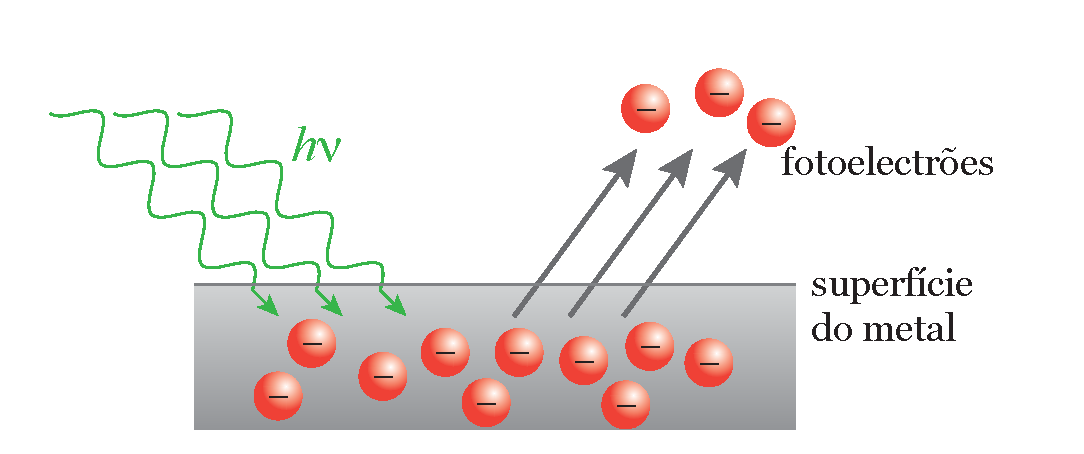
\includegraphics[width=0.65\textwidth]{./planck_images/pe-effect.pdf}
	\caption{Ilustração do efeito fotoeléctrico} \label{fig:pe-effect}
\end{figure}

A constante de Planck pode ser determinada expondo a superfície de um metal a luz monocromática, caracterizada por um
comprimento de onda $\lambda=c /\nu$ fixo e medindo a energia cinética máxima dos fotoelectrões emitidos. A Fig.~\ref{fig:plack_exp}
representa esquematicamente uma montagem experimental para a realização desta experiência.

\begin{figure}[htb] 
	\centering 
	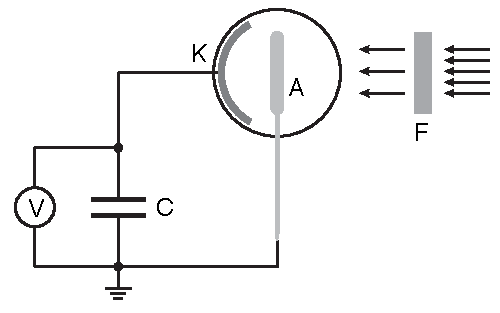
\includegraphics[width=0.5\textwidth]{./planck_images/planck_exp.pdf}
	\caption{Diagrama esquemático da experiência do efeito fotoeléctrico. V - fonte de tensão (potencial retardador);
	C - condensador; K - cátodo; A - ânodo; F - filtro óptico.} \label{fig:plack_exp}
\end{figure}
A luz incide na superfície de um sólido metálico, designado \emph{cátodo} (K), através de um \emph{ânodo} (A) anelar ou transparente. 
Como cátodo, é normalmente utilizado um metal alcalino (potássio, sódio ou cádmio)  pois neste caso os electrões de valência estão
fracamente 
ligados ao núcleo (i.e. têm uma baixa função trabalho $W_0$). Como ânodo, utiliza-se por exemplo a platina (Pt). 
O ânodo recebe parte dos fotoelectrões emitidos, dando origem a uma corrente $I_f$ no circuito exterior. 
Se aplicarmos um potencial eléctrico retardador $V$ entre o ânodo e o cátodo a fotocorrente decresce, pois os fotoelectrões
terão de vencer uma barreira de potencial electrostática $U=e V$, onde $e$ é a carga do electrão. 
Para uma dada tensão crítica $V_s$ (potencial de paragem), deixa de existir fotocorrente. 
%Neste caso, mesmo os electrões mais fracamente ligados e que assim têm as maiores energias cinéticas, são parados. 

%$I_f=C\frac{dq}{dt}$
Experimentalmente, pode usar-se uma fonte de tensão externa para aplicar o potencial de paragem. Mais simplesmente,
pode usar-se um condensador para acumular a carga ($q=C V$) transportada pela própria corrente dos fotoelectrões (Fig.~\ref{fig:plack_exp}),
aumentando gradualmente a diferença de potencial $V$, até se atingir o valor $V_s$, para o qual a corrente é  auto-eliminada.
Mas neste caso, é necessário utilizar um voltímetro de impedância de entrada muito elevada ($> 10\textrm{ M}\Omega$) ou um
amplificador electrónico de instrumentação, que é o caso da nossa montagem experimental.
 Após medir o potencial de paragem, podemos assim escrever:\footnote{Na realidade a função de trabalho tem de ser corrigida
 pelo potencial de contacto entre os dois metais, $W=W_0 - \phi$, o que naturalmente não é importante para a determinação da
 constante de proporcionalidade.}
\begin{equation}
	\label{eq:energia}
	e\,V_s= K_e^{max}= h \nu - W_O
\end{equation}
Medindo o potencial de paragem sucessivamente para luz incidente de várias frequências, podemos então fazer o gráfico de
$V_s\; vs. \;\nu$. Este gráfico deverá aproximar-se de uma recta de declive $h/e$ e ordenada na origem  $-W_0/e$
(ver exemplo na Fig. \ref{fig:pe-graph}).


\begin{figure}[htb] 
	\centering 
	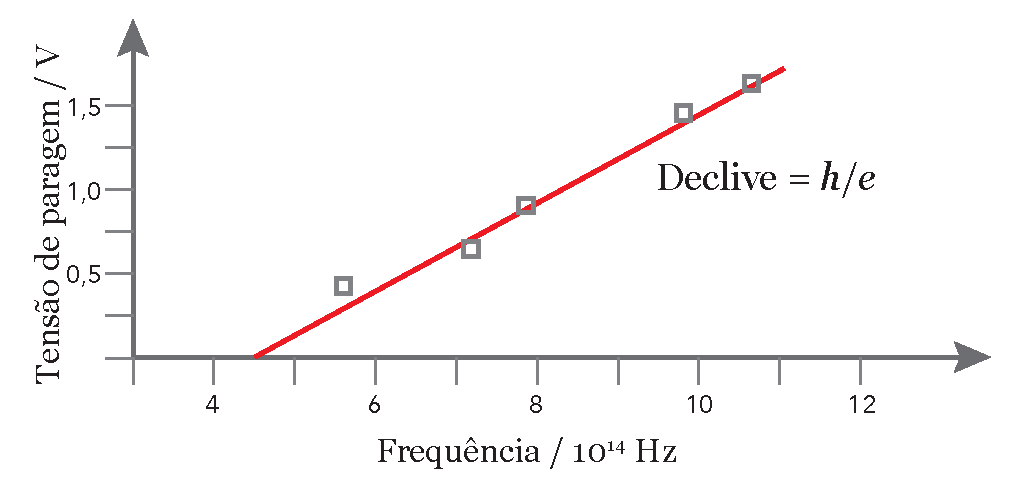
\includegraphics[width=0.65\textwidth]{./planck_images/pe-graph.pdf}
	\caption{Exemplo da determinação de $h$ pelo efeito fotoeléctrico} \label{fig:pe-graph}
\end{figure}

Desde a redefinição do Sistema Internacional de Unidades de 2019, a constante $h$ é definida como tendo um valor exacto:
$h=6.626\,070\,15 \times 10^{-34}\ \textrm{J}\cdot \textrm{s}$ ou, em unidades de electrão-volt,
$h=4.135\,667\,696\times 10^{-15}\,\textrm{eV}\cdot\textrm{s}$. No âmbito do SI, a constante de Planck é usada na definição
do quilograma.

\newpage
 \subsection{\sf Figuras dos aparelhos da montagem experimental}
 \begin{figure}[htb] 
	\centering 
	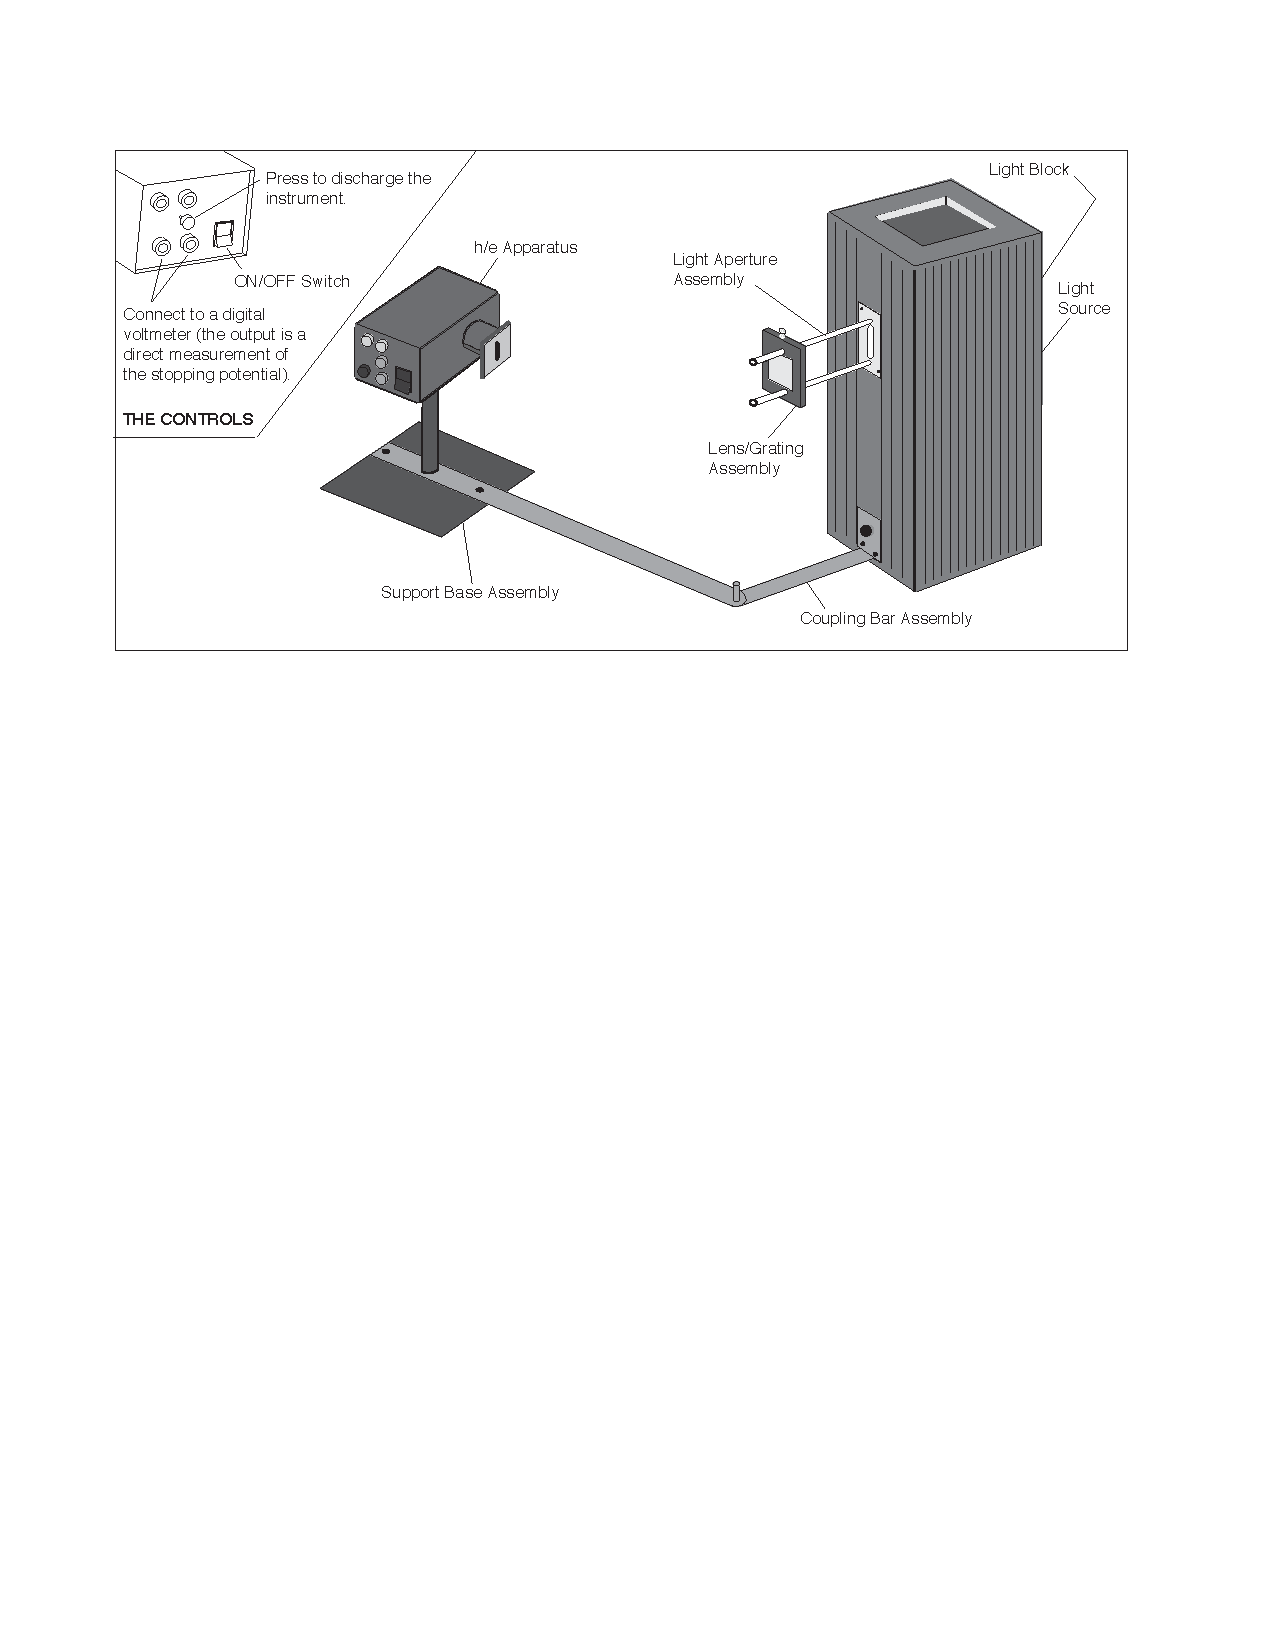
\includegraphics[width=0.9\textwidth]{./planck_images/planckPasco} 
	\caption{Montagem experimental do efeito fotoeléctrico - esquema} 
	\label{fig:plackPasco}
\end{figure}

 \begin{figure}[htb] 
	\centering 
	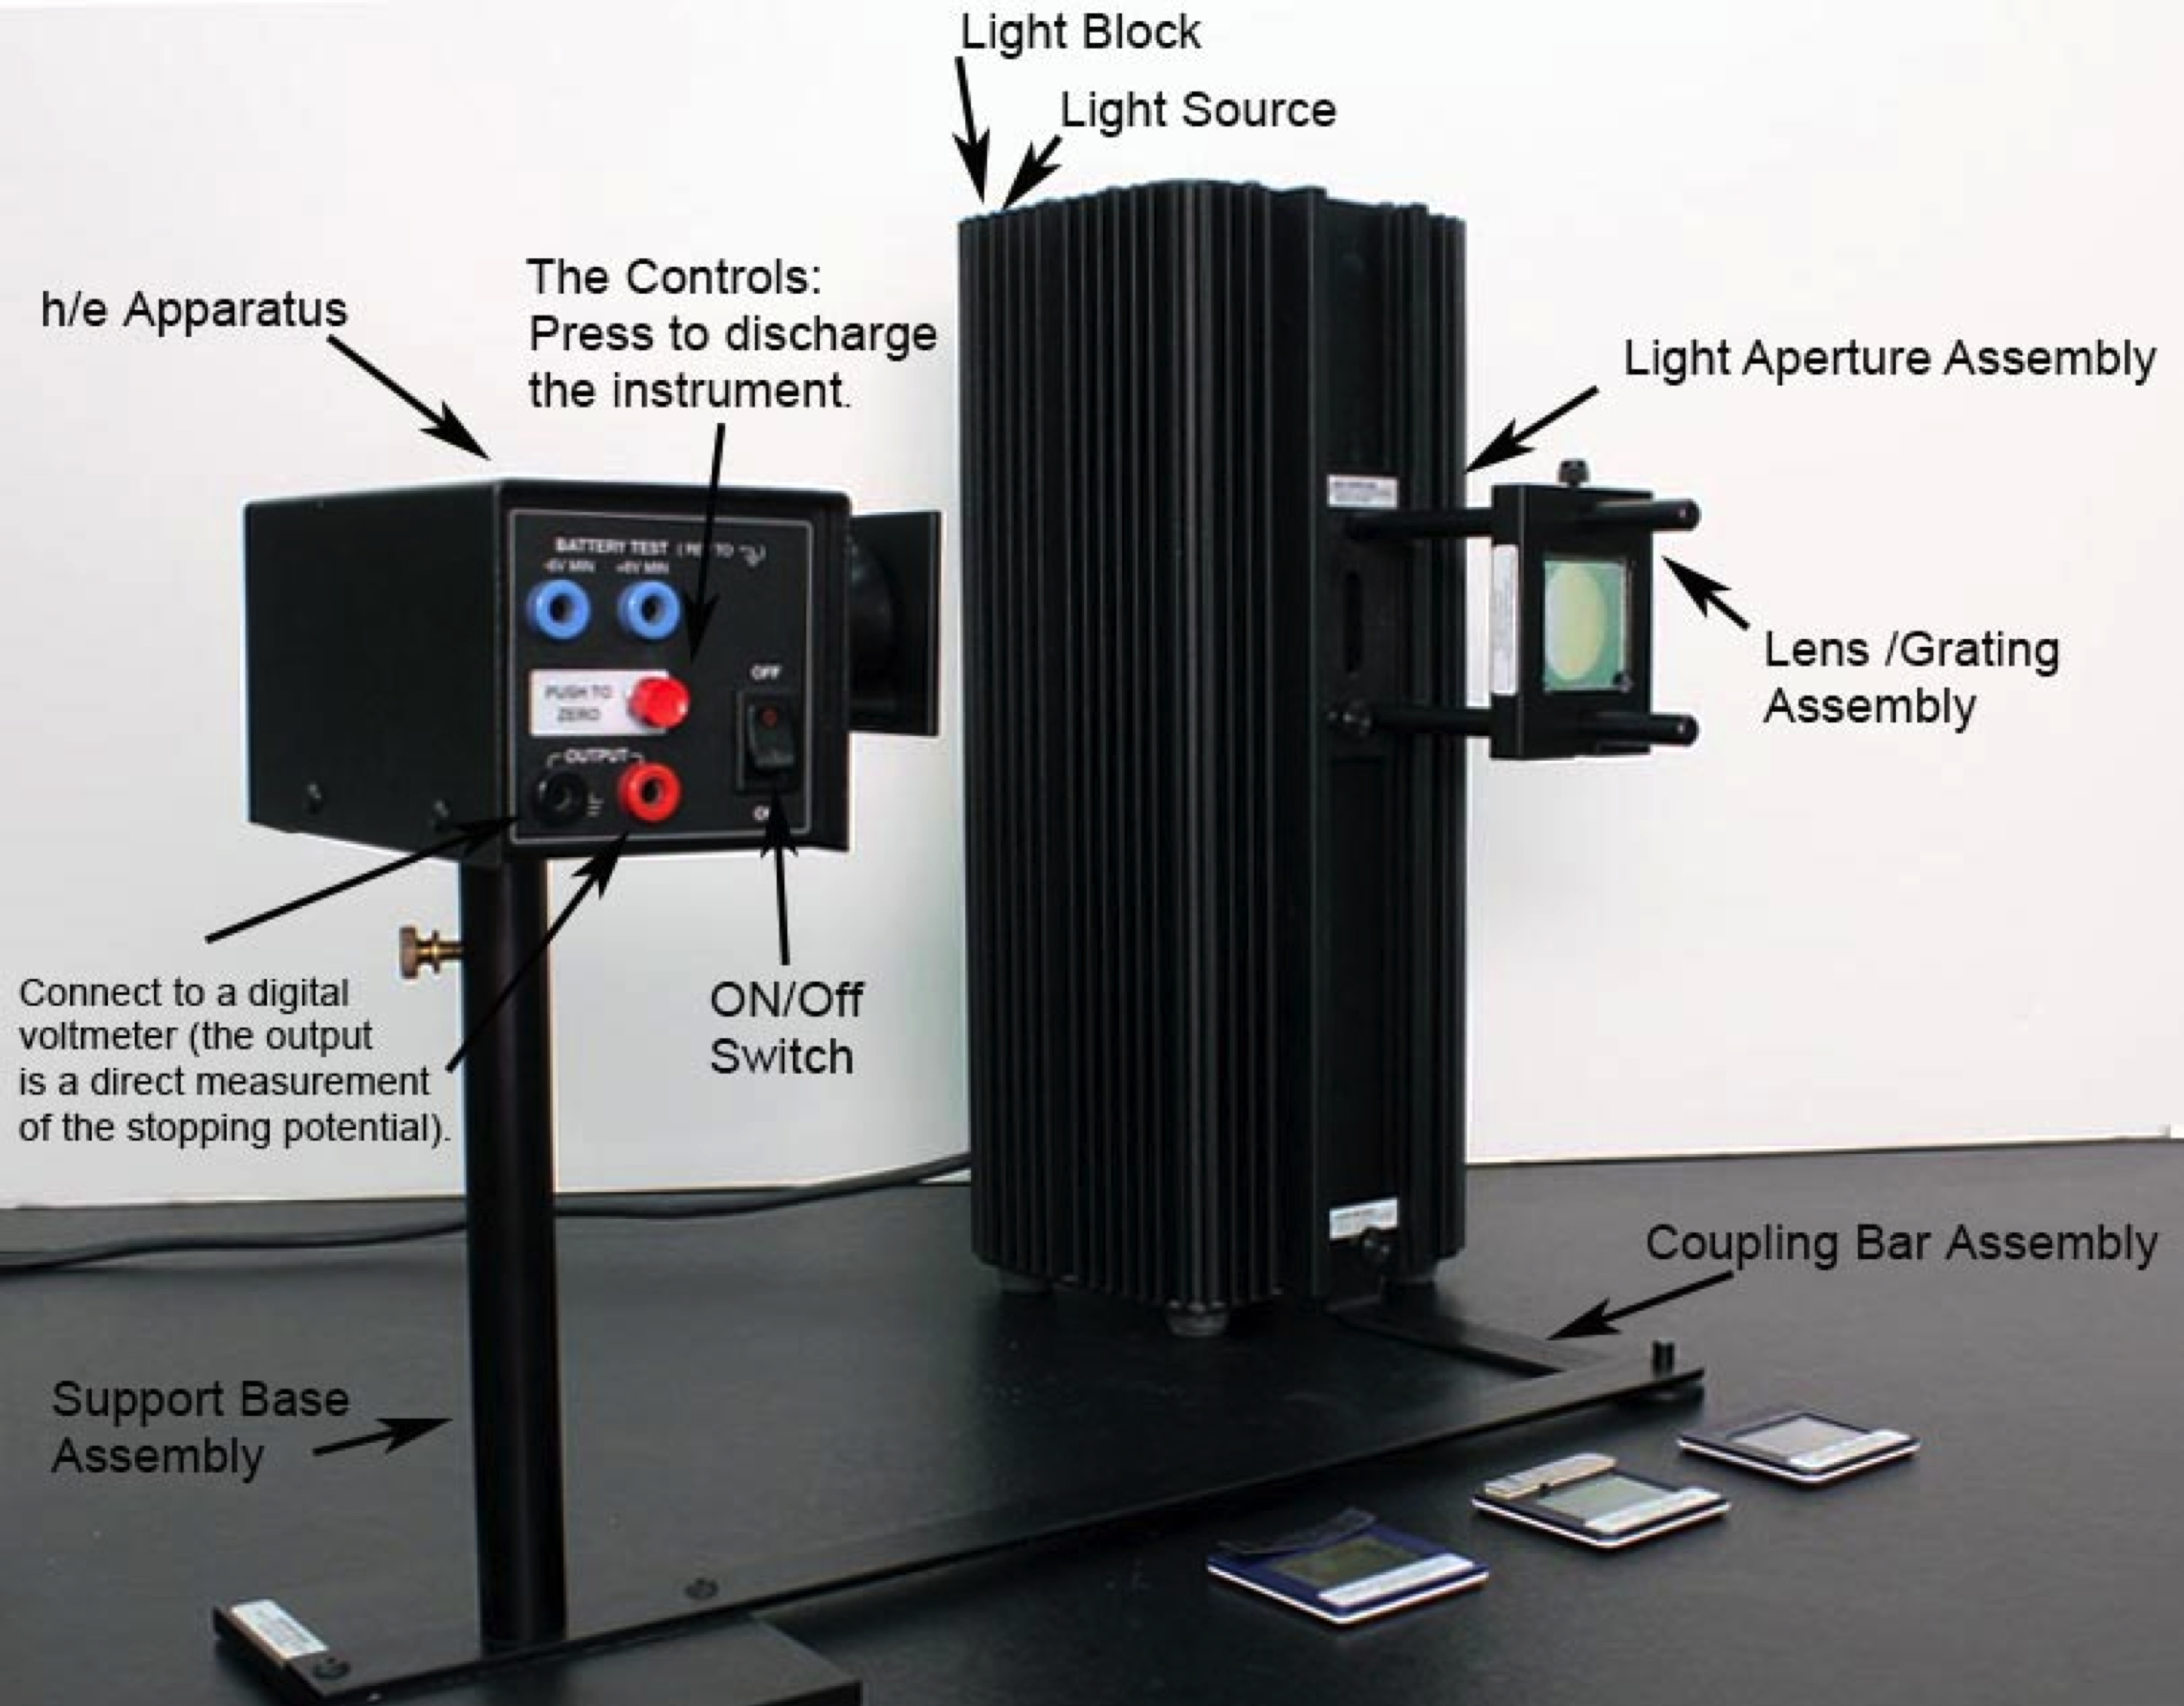
\includegraphics[width=0.65\textwidth]{./planck_images/Planck_setup} 
	\caption{Montagem experimental do efeito fotoeléctrico - fotografia} 
\end{figure}

%%%%%%%%%%%%%%%
\newpage
\section{\sf Procedimento experimental}

\subsection{\sf Trabalho preparatório} 
\begin{enumerate}
\item Preencha os objectivos do trabalho que irá realizar na sessão de laboratório. 
\item Preencha o quadro com as equações necessárias para o cálculo das grandezas, bem como as suas incertezas. 
\end{enumerate}

\subsection{\sf Goniómetro}

\subsection*{\sf Material utilizado}

\begin{itemize}
\item goniómetro
\item fonte de luz incandescente (candeeiro)
\item luz espectral de Hg ou He
\item prisma
\item rede de difração
\item nível graduado
\end{itemize}

\fbox{\begin{minipage}{35em}
\textbf{Atenção:} Este trabalho envolve o uso de lâmpadas espectrais. Estas lâmpadas são uma fonte de radiação ultravioleta,
que tem efeitos nocivos nos olhos e na pele. Apesar das lâmpadas existentes no laboratório terem uma potência de emissão
relativamente baixa, deve-se evitar a exposição desnecessária ou a observação prolongada da sua luz.
\end{minipage}}
\\

\subsection*{\sf Alinhamento do goniómetro}
\begin{enumerate}
%\item Ligue  a  lâmpada  espetral  e  espere  10  a  15  minutos    %até  que  se  estabeleça  o 
%equilíbrio térmico no seu interior. 
\item Disponha o goniómetro em frente a uma fonte luminosa de luz incandescente. Entretanto, ligue também a fonte de luz
espectral, de modo a permitir que se estabilize termicamente (10 a 15 minutos).
\item Comece por regular a ocular da luneta. Para isso, deve ver nitidamente com um olho  os fios do retículo e simultaneamente
com o outro olho ver um objecto no exterior da luneta, afastado a cerca de 30 cm.  
\item Para  regular  a  objectiva,  observe  agora  um  objecto  no  “infinito” (no  laboratório, escolha  um objecto o mais
afastado possível)  actuando  sobre  o  parafuso  da  luneta.  Regule  de  modo  a observar o objecto e o retículo, bem focado
e sem paralaxe. 
\item Coloque  a  luneta  alinhada de frente  para o  colimador  e  regule o parafuso deste, de modo a observar a fenda
focada quando iluminada pela lâmpada espectral. 
\item Com o nível de bolha, verifique a horizontalidade do goniómetro e da plataforma.
\item \underline{Muito importante -- antes de começar as medições:} 
\begin{itemize}
\item Identifique as escalas dos ângulos usados para medir a orientação da plataforma e da luneta. Note que a escala de graus
varia de $0^\circ$ a $360^\circ$ e depois recomeça, pelo que poderá ser necessário fazer a conversão adequada caso a gama de
valores medidos contenha esta transição. 
\item Assegure-se de que compreende como estão relacionadas as duas escalas opostas e como funcionam os nónios. A leitura
dos valores dos nónios é facilitada com o auxílio de uma lupa -- use uma das lentes convergentes.
\end{itemize}
\end{enumerate}

\subsection*{\sf Rede de difracção}
A variação do desvio angular com o c.d.o. é significativa no caso da rede de difracção, pelo que para esta medição basta
usar a escala principal (em graus) do goniómetro.

\begin{enumerate}
	\item Antes de colocar a rede, comece por alinhar a luneta com o colimador e registe o valor do ângulo $\phi_{t0}$ lido
	na escala da luneta.
	\item Monte no centro da plataforma do goniómetro uma rede de difração de 600 linhas por milímetro, orientada com uma das
	faces de frente para o colimador, isto é, de modo a que o feixe incida o mais possível na perpendicular à superfície da rede.
	\item Substitua a lâmpada incandescente pela fonte de luz espectral. Observe os raios difractados de várias cores, em 1.ª e 2.ª ordem. Meça e registe o ângulo de transmissão $\phi_t$ de todas as riscas espectrais que conseguir observar, com a melhor precisão possível, à esquerda e à direita da ordem central $m=0$.
	\item Identifique os diversos comprimentos de onda e compare com os valores tabelados para a lâmpada espectral que está a utilizar. No final, retire a rede de difracção.
\end{enumerate}

\subsection*{\sf Prisma}
A variação do desvio angular com o c.d.o. é muito ténue no caso do prisma, pelo que para esta medição é essencial recorrer
à escala principal e ao nónio do goniómetro. 

\begin{enumerate}
\item Antes de colocar o prisma, volte a alinhar a luneta com o colimador e registe o valor do ângulo $\phi_0$ lido na escala
da luneta.
\item Rode a plataforma de modo a obter na respectiva escala a leitura $\phi_i=0^\circ$.
\item Cuidadosamente, monte no centro da plataforma um prisma (de ângulo de vértice conhecido), orientado com uma das faces de
frente para o colimador, isto é, de modo a que o feixe incida o mais possível na perpendicular à superfície do prisma.
\item Rode agora o prisma de modo a obter uma configuração semelhante à da Fig. \ref{fig:babinet}, prestando atenção à orientação
correcta do vértice e da direcção da luz refractada, que deverá ser visível mesmo sem o auxílio da luneta.
\item  Na luneta, observe as várias cores refractadas.  Se o instrumento estiver bem focado, deverá  observar  uma  série  de
imagens coloridas da fenda (riscas verticais), uma por cada comprimento de onda. Escolha duas cores, bem afastadas. 
\item Para uma das cores, rode suavemente a plataforma até encontrar a configuração para o qual se regista o desvio mínimo.
Nessa posição, centre no retículo a risca observada e registe o valor de $\phi_{i,min}$ (escala da plataforma), bem como o
respectivo ângulo de transmissão $\phi_{t,min}$ (escala da luneta).
\item Realize um conjunto de dez pares de leituras $(\phi_i,\phi_t)$: cinco para ângulos de incidência inferiores a $\phi_{i,min}$ e cinco para ângulos de incidência superiores, preenchendo a tabela. Mais uma vez, note que para estas medições é essencial o uso do nónio em ambas as escalas.
\item Repita os pontos 17 e 18 para a risca da outra cor. 
\item Para cada cor, elabore um gráfico dos ângulos de desvio $\delta$ em função de $\phi_i$ e anexe-os ao relatório. Realize
um ajuste polinomial e verifique que tanto o ângulo de desvio mínimo como a curva obtida são diferentes para cada cor.
\item Usando a Eq. (5.1) com $\alpha=30^\circ$, determine o valor do índice de refracção para os dois c.d.o. que utilizou.
\end{enumerate}


\newpage
\subsection{\sf Efeito fotoeléctrico}
\subsection*{\sf Parte I. Laboratório presencial}
\fbox{\begin{minipage}{35em}
\textbf{Atenção:} este trabalho envolve o uso de lâmpadas espectrais. Estas lâmpadas são uma fonte de radiação ultravioleta,
que tem efeitos nocivos nos olhos e na pele. Apesar das lâmpadas existentes no laboratório terem uma potência de emissão
relativamente baixa, deve-se evitar a exposição desnecessária ou a observação prolongada da sua luz.
\end{minipage}}\\ \\


\begin{enumerate}
\item Ligue a fonte da lâmpada de mercúrio e deixe estabilizar durante cerca de 10 minutos.
\item Enquanto espera, teste as tensões de cada uma das duas pilhas do amplificador da célula fotovoltaica.
\item Monte os componentes tal como indicado na Fig.~\ref{fig:plackPasco}.
\item Regule o conjunto de lente + rede de difracção de modo a obter as riscas de cor bem focadas na zona do detector.
Alinhe a montagem da fenda para que a célula esteja bem iluminada e centrada na risca.
\item O que observa depois da rede é uma \emph{figura de difracção}. 
%Observe as várias riscas, anote e interprete os ângulos de Difração e Ordem. 
Esta figura é simétrica (esquerda/direita) no que respeita às posições das riscas e das intensidades observadas? Quantas
ordens de difracção consegue identificar?
\item Para cada uma das riscas (cores) pressione o botão de RESET e depois registe o valor da tensão de paragem $V_s$. Faça
três medidas para cada risca. Note que para as riscas amarela e verde é necessário utilizar os respectivos filtros coloridos.
\end{enumerate}

\begin{table}[!hbp]
\begin{center}
	%\centering
	\begin{tabular}{|c|c|c|}
	\hline
	Cor  & Freq. [THz] & $\lambda$ [nm]  \\
	\hline
	Amarelo & 518.672 & 578 \\
	Verde & 548.996 & 546.074\\
	Azul & 687.858  & 435.835 \\
	Violeta & 740.858  & 404.656\\
	U.V.    & 820.264  & 365.483 \\
	\hline
 	\end{tabular}
	\caption{Riscas observáveis do espectro da lâmpada de Hg. No material de apoio de LIFE pode encontrar informação sobre
	as principais riscas espectrais deste e de outros elementos.} 
	\label{tab:Hg}
	\end{center}
\end{table}

\subsubsection*{\sf Determinação da recta de ajuste}
\underline{Ajuste manual} -- Usando o quadriculado disponibilizado, faça o gráfico de $V_s$ em função da frequência $\nu$.
Escolha os eixos adequadamente e complete o gráfico (com título, unidades, escala, marcas, etc.). Deverá tentar aproveitar
ao máximo a área útil da folha, de modo a minimizar as incertezas. Com uma régua, tente ajustar uma recta $(y=mx + b)$ aos
pontos experimentais e determine o seu declive, a  abcissa na origem (a.o.) e a suas incertezas. Consulte o \emph{Material de apoio}
de LIFE para este procedimento.\\
\underline{Ajuste através de software} -- Faça o ajuste numérico com o auxílio de software adequado (\emph{Fitteia}, calculadora
gráfica, Gnuplot, etc.) 


\subsection*{\sf Parte II. Laboratório remoto}
O laboratório remoto \emph{e-lab} permite obter o potencial de paragem para diferentes riscas e diferentes níveis de intensidade,
permitindo ainda registar a variação da curva ao longo do tempo. Esta componente pode ser realizada a partir de um computador
pessoal, não sendo necessário estar no laboratório.\\

\begin{enumerate}
\item Para realizar a experiência remota,  aceda à lista de experiências do \emph{e-lab} em\\
\texttt{http://elab.ist.utl.pt/rec.web//}\\
e siga as instruções transmitidas no MOOC de LIFE.
\item Para seguir o protocolo experimental, aceda a\\ 
\texttt{http://www.elab.tecnico.ulisboa.pt/wiki/index.php}\\
e seleccione a experiência "Determinação da Constante de Planck". Realize as medições e análises descritas na secção "Protocolo".
\end{enumerate}

	
\newpage
\def\width{15}
\def\hauteur{25}
\begin{tikzpicture}[x=1cm, y=1cm, semitransparent]
\draw[step=1mm, line width=0.1mm, black!30!white] (0,0) grid (\width,\hauteur);
\draw[step=5mm, line width=0.2mm, black!40!white] (0,0) grid (\width,\hauteur);
\draw[step=5cm, line width=0.5mm, black!50!white] (0,0) grid (\width,\hauteur);
\draw[step=1cm, line width=0.3mm, black!90!white] (0,0) grid (\width,\hauteur);
\end{tikzpicture}


\newpage

\end{document}